\documentclass[tikz, border=5mm]{standalone}
\usepackage[utf8]{inputenc}
\usepackage{amsmath}
\usepackage{amssymb}
\usetikzlibrary{shapes.geometric, arrows.meta, positioning, calc}

\begin{document}
% TIPP: Um das Diagramm in deinem Hauptdokument perfekt auf A4 anzupassen,
% kannst du es mit \resizebox{!}{0.95\textheight}{ \begin{tikzpicture} ... \end{tikzpicture} } einbinden.

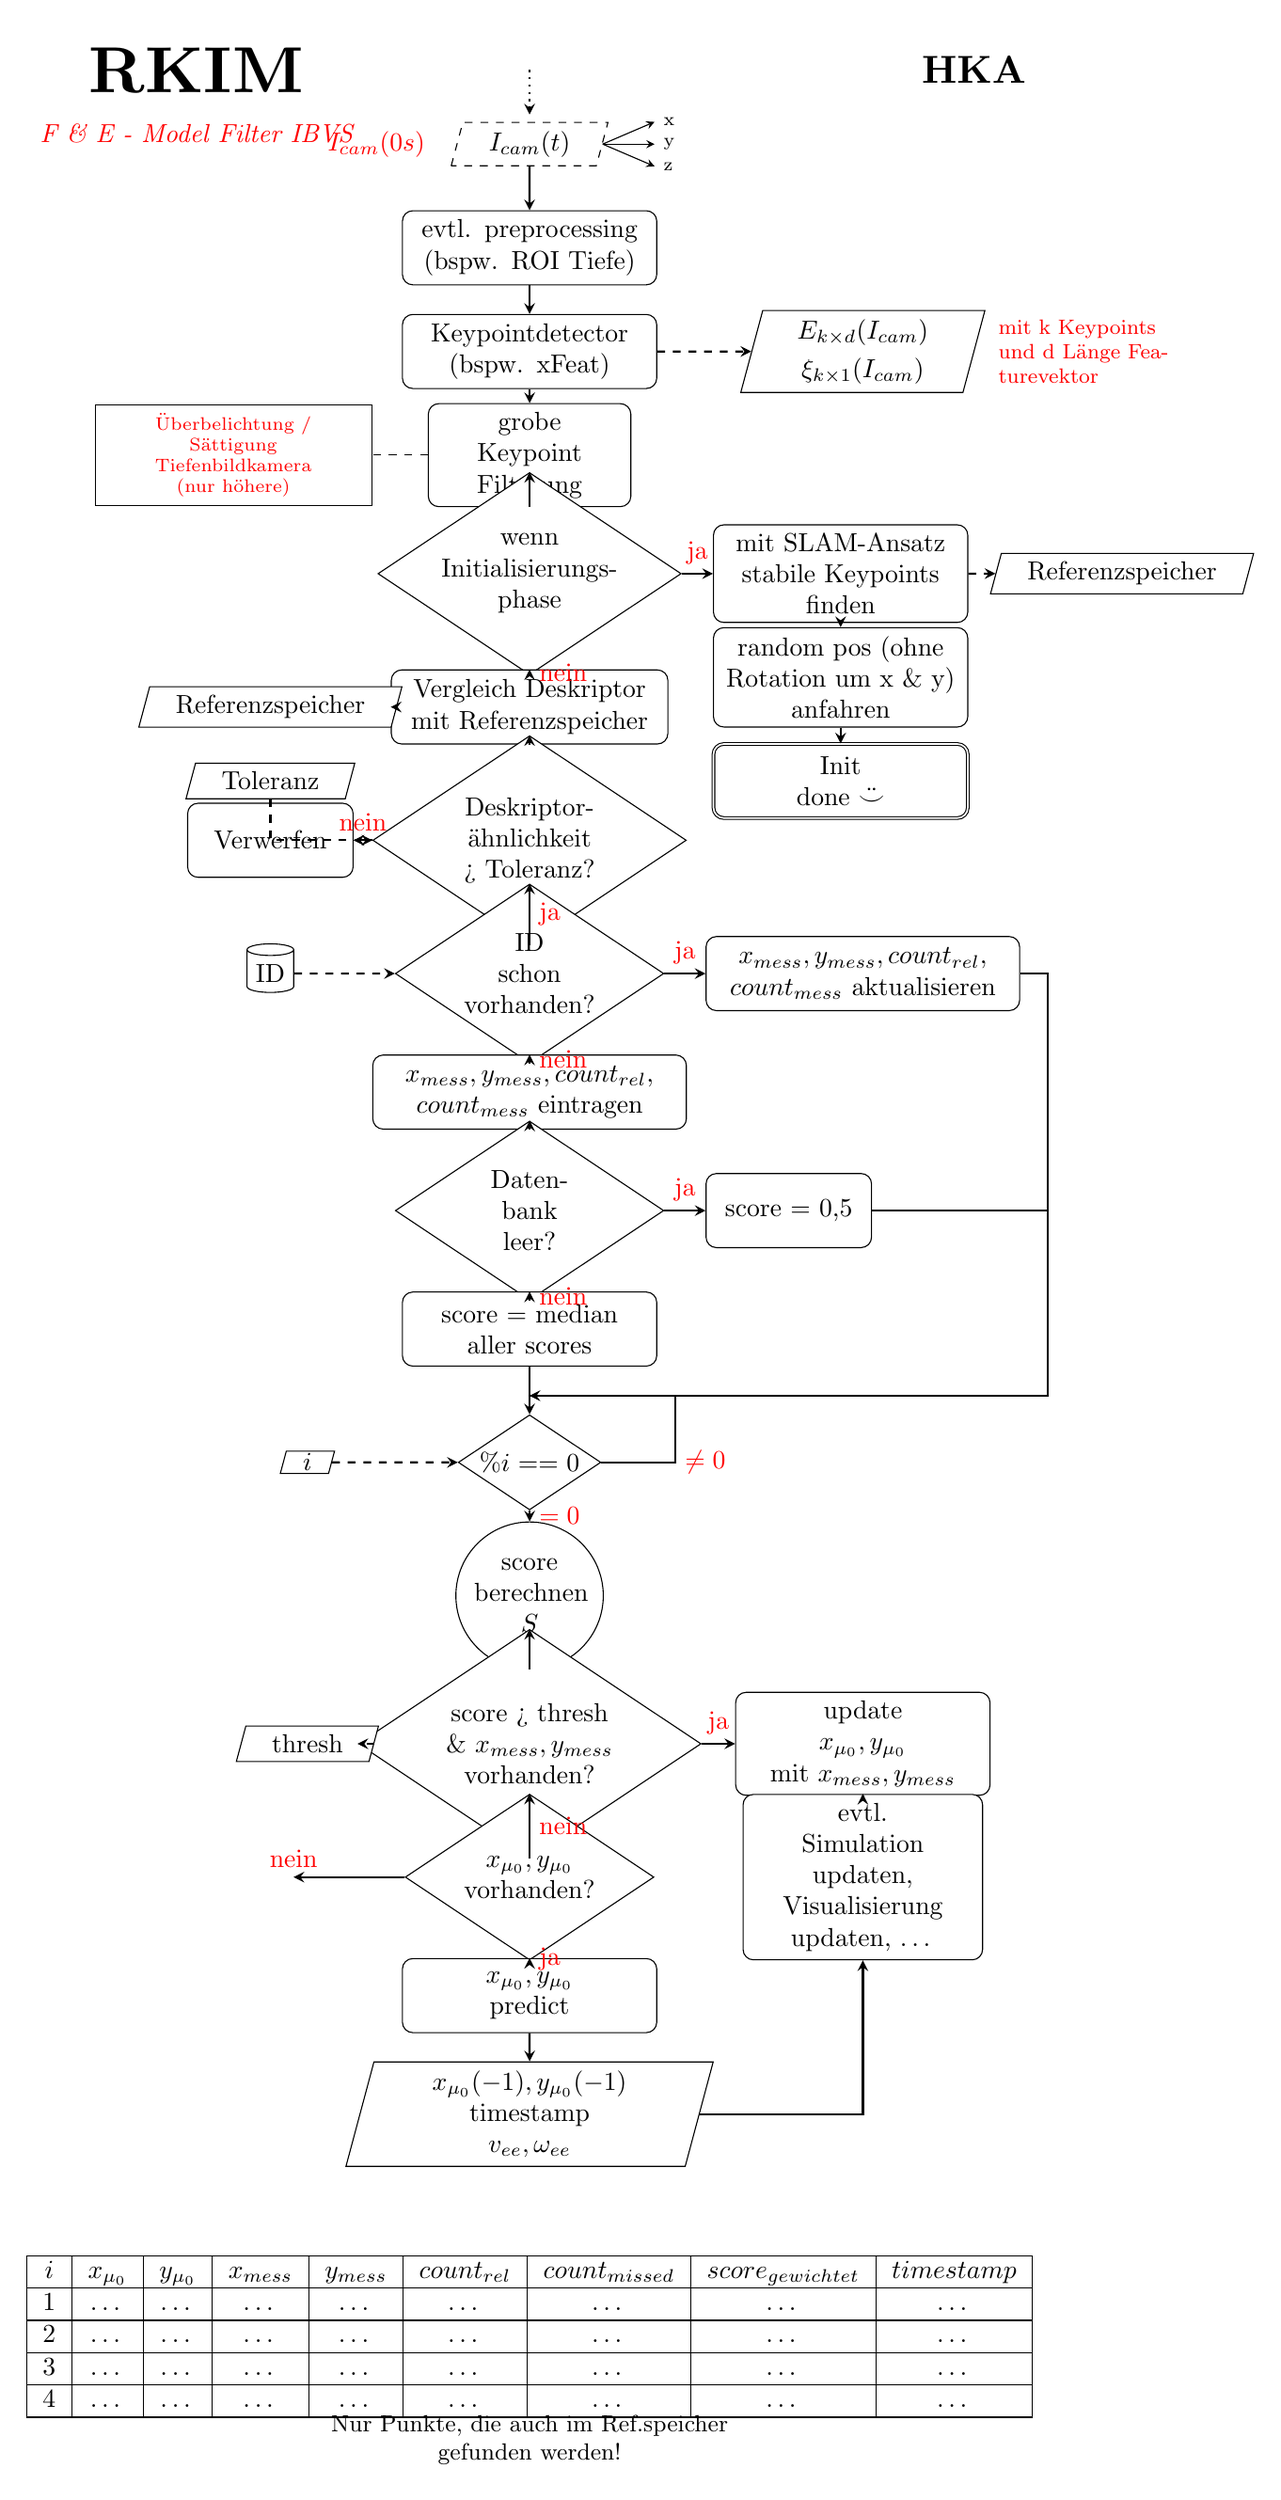
\begin{tikzpicture}[
    >=stealth,
    % Definition der Stile
    process/.style={rectangle, draw=black, rounded corners, text centered, text width=3.2cm, minimum height=1cm, fill=white},
    decision/.style={diamond, draw=black, text centered, text width=2cm, aspect=1.5, fill=white, inner sep=0pt},
    io/.style={trapezium, trapezium left angle=75, trapezium right angle=105, draw=black, text centered, fill=white, inner xsep=10pt},
    db/.style={cylinder, draw=black, shape border rotate=90, aspect=0.25, text centered, fill=white},
    circleop/.style={circle, draw=black, text centered, inner sep=2pt, fill=white},
    arrow/.style={->, thick},
    dashedarrow/.style={->, thick, dashed},
    line/.style={thick}
]

    % ==========================================
    % HEADER
    % ==========================================
    \node[scale=2.5, font=\bfseries] (rkim) at (-4.5, 0) {RKIM};
    \node[text=red, font=\itshape, anchor=north] at (rkim.south) {F \& E - Model Filter IBVS};
    \node[scale=1.5, font=\bfseries] at (6, 0) {HKA};

    % ==========================================
    % MAIN VERTICAL FLOW (Center Column x=0)
    % ==========================================
    
    % Input & Preprocessing
    \draw[arrow, dotted] (0, 0) -- (0, -0.6);
    \node[io, dashed] (Icam) at (0, -1.0) {$I_{cam}(t)$};
    \node[text=red, left=0.3cm of Icam] {$I_{cam}(0s)$};
    
    % Koordinaten-Pfeile an Icam
    \draw[->] (Icam.east) -- ++(0.7, 0.3) node[right, font=\scriptsize] {x};
    \draw[->] (Icam.east) -- ++(0.7, 0) node[right, font=\scriptsize] {y};
    \draw[->] (Icam.east) -- ++(0.7, -0.3) node[right, font=\scriptsize] {z};

    \node[process] (preproc) at (0, -2.4) {evtl. preprocessing\\(bspw. ROI Tiefe)};
    \node[process] (keypoint) at (0, -3.8) {Keypointdetector\\(bspw. xFeat)};
    \node[process, text width=2.5cm] (filter) at (0, -5.2) {grobe\\Keypoint Filterung};
    \node[decision, text width=2.5cm] (initdec) at (0, -6.8) {wenn\\Initialisierungs-\\phase};
    \node[process, text width=3.5cm] (compare) at (0, -8.6) {Vergleich Deskriptor\\mit Referenzspeicher};
    \node[decision, text width=2.5cm] (simdec) at (0, -10.4) {Deskriptor-\\ähnlichkeit\\> Toleranz?};
    \node[decision] (iddec) at (0, -12.2) {ID\\schon\\vorhanden?};
    \node[process, text width=4cm] (insertid) at (0, -13.8) {$x_{mess}, y_{mess}, count_{rel},$\\$count_{mess}$ eintragen};
    \node[decision] (dbdec) at (0, -15.4) {Daten-\\bank\\leer?};
    \node[process] (scoremed) at (0, -17.0) {score = median\\aller scores};
    
    % Modulo & Score (Merges happen before moddec)
    \node[decision, text width=1.5cm] (moddec) at (0, -18.8) {$\% i == 0$};
    \node[circleop, text width=1.5cm] (calc) at (0, -20.6) {score\\berechnen\\$S$};
    
    % Threshold & Endings
    \node[decision, text width=3cm] (threshdec) at (0, -22.6) {score > thresh\\\& $x_{mess}, y_{mess}$\\vorhanden?};
    \node[decision, text width=2.5cm] (mudec) at (0, -24.4) {$x_{\mu_0}, y_{\mu_0}$\\vorhanden?};
    \node[process] (predict) at (0, -26.0) {$x_{\mu_0}, y_{\mu_0}$\\predict};
    \node[io, text width=3.5cm] (preddata) at (0, -27.6) {$x_{\mu_0}(-1), y_{\mu_0}(-1)$\\timestamp\\$v_{ee}, \omega_{ee}$};


    % ==========================================
    % SIDE ELEMENTS & BRANCHES
    % ==========================================
    
    % Matrix rechts neben Keypoint
    \node[io, text width=2cm] (mat) at (4.5, -3.8) {$E_{k \times d}(I_{cam})$\\[1mm] $\xi_{k \times 1}(I_{cam})$};
    \node[right=0.2cm of mat, text=red, font=\footnotesize, text width=2.5cm, align=left] {mit k Keypoints\\und d Länge Featurevektor};
    
    % Filterinfo links
    \node[draw=black, text=red, font=\scriptsize, text width=3.5cm, align=center] (filterinfo) at (-4, -5.2) {Überbelichtung /\\Sättigung\\Tiefenbildkamera\\(nur höhere)};
    
    % Init Phase (Rechter Zweig)
    \node[process] (slam) at (4.2, -6.8) {mit SLAM-Ansatz\\stabile Keypoints\\finden};
    \node[io] (ref1) at (8.0, -6.8) {Referenzspeicher};
    \node[process] (randpos) at (4.2, -8.2) {random pos (ohne\\Rotation um x \& y)\\anfahren};
    \node[process, double] (initdone) at (4.2, -9.6) {Init\\done $\ddot{\smile}$};
    
    % Referenzspeicher & Toleranz (Links)
    \node[io] (ref2) at (-3.5, -8.6) {Referenzspeicher};
    \node[io] (tol) at (-3.5, -9.6) {Toleranz};
    \node[process, text width=2cm] (discard) at (-3.5, -10.4) {Verwerfen};
    
    % ID Datenbank (Links)
    \node[db] (iddb) at (-3.5, -12.2) {ID};
    
    % Update Branch (Rechts)
    \node[process, text width=4cm] (updateid) at (4.5, -12.2) {$x_{mess}, y_{mess}, count_{rel},$\\$count_{mess}$ aktualisieren};
    
    % Score 0,5 (Rechts)
    \node[process, text width=2cm] (score5) at (3.5, -15.4) {score = 0,5};
    
    % Loop "i" (Links)
    \node[io, inner sep=1pt, text width=0.5cm] (iloop) at (-3.0, -18.8) {$i$};
    
    % Thresh input (Links)
    \node[io] (thresh) at (-3.0, -22.6) {thresh};
    
    % Update Simulation branches (Rechts)
    \node[process] (updatemu) at (4.5, -22.6) {update\\$x_{\mu_0}, y_{\mu_0}$\\mit $x_{mess}, y_{mess}$};
    \node[process, text width=3cm] (simup) at (4.5, -24.4) {evtl.\\Simulation\\updaten,\\Visualisierung\\updaten, \dots};


    % ==========================================
    % VERBINDUNGEN (ARROWS)
    % ==========================================

    % Hauptachse Oben
    \draw[arrow] (Icam) -- (preproc);
    \draw[arrow] (preproc) -- (keypoint);
    \draw[dashedarrow] (keypoint) -- (mat);
    \draw[arrow] (keypoint) -- (filter);
    \draw[dashed] (filter) -- (filterinfo);
    \draw[arrow] (filter) -- (initdec);

    % Init Phase
    \draw[arrow] (initdec) -- node[above, text=red] {ja} (slam);
    \draw[dashedarrow] (slam) -- (ref1);
    \draw[arrow] (slam) -- (randpos);
    \draw[arrow] (randpos) -- (initdone);
    \draw[arrow] (initdec) -- node[right, text=red] {nein} (compare);

    % Vergleich & Matching
    \draw[dashedarrow] (ref2) -- (compare);
    \draw[arrow] (compare) -- (simdec);
    \draw[dashedarrow] (tol.south) |- (simdec.west);
    \draw[arrow] (simdec) -- node[above, text=red] {nein} (discard);
    
    % ID Abfrage
    \draw[arrow] (simdec) -- node[right, text=red] {ja} (iddec);
    \draw[dashedarrow] (iddb) -- (iddec);
    \draw[arrow] (iddec) -- node[above, text=red] {ja} (updateid);
    \draw[arrow] (iddec) -- node[right, text=red] {nein} (insertid);

    % Datenbank Check
    \draw[arrow] (insertid) -- (dbdec);
    \draw[arrow] (dbdec) -- node[above, text=red] {ja} (score5);
    \draw[arrow] (dbdec) -- node[right, text=red] {nein} (scoremed);

    % --- MERGE POINT ---
    % Alle Pfade (scoremed, score5, updateid) fließen auf y=-17.9 zusammen
    \coordinate (merge_point) at (0, -17.9);
    \draw[line] (scoremed.south) -- (merge_point);
    % Updateid wird ganz außen rechts geführt, um score5 nicht zu kreuzen
    \draw[line] (updateid.east) -| (7, -17.9) -- (merge_point);
    \draw[line] (score5.east) -| (7, -17.9);
    \draw[arrow] (merge_point) -- (moddec.north);

    % Modulo Check & Loop
    \draw[dashedarrow] (iloop) -- (moddec);
    \draw[arrow] (moddec) -- node[right, text=red] {$=0$} (calc);
    \draw[arrow] (moddec.east) -- ++(1,0) node[right, text=red] {$\neq 0$} |- (merge_point);

    % Calculate & Threshold
    \draw[arrow] (calc) -- (threshdec);
    \draw[dashedarrow] (thresh) -- (threshdec);
    
    \draw[arrow] (threshdec) -- node[above, text=red] {ja} (updatemu);
    \draw[arrow] (updatemu) -- (simup);

    % Prediction Branch
    \draw[arrow] (threshdec) -- node[right, text=red] {nein} (mudec);
    \draw[arrow] (mudec) -- node[right, text=red] {ja} (predict);
    \draw[arrow] (mudec.west) -- ++(-1.5,0) node[above, text=red] {nein};
    \draw[arrow] (predict) -- (preddata);
    
    % Return Path from Preddata to Simup
    \draw[arrow] (preddata.east) -| (simup.south);


    % ==========================================
    % TABELLE (Unten zentriert)
    % ==========================================
    \node[anchor=north, inner sep=0pt] (table) at (0, -29.5) {
        \begin{tabular}{|c|c|c|c|c|c|c|c|c|}
        \hline
        $i$ & $x_{\mu_0}$ & $y_{\mu_0}$ & $x_{mess}$ & $y_{mess}$ & $count_{rel}$ & $count_{missed}$ & $score_{gewichtet}$ & $timestamp$ \\
        \hline
        1 & \dots & \dots & \dots & \dots & \dots & \dots & \dots & \dots \\
        \hline
        2 & \dots & \dots & \dots & \dots & \dots & \dots & \dots & \dots \\
        \hline
        3 & \dots & \dots & \dots & \dots & \dots & \dots & \dots & \dots \\
        \hline
        4 & \dots & \dots & \dots & \dots & \dots & \dots & \dots & \dots \\
        \hline
        \end{tabular}
    };
    \node[text=black, font=\small, align=center] at (0, -32) {Nur Punkte, die auch im Ref.speicher\\gefunden werden!};

\end{tikzpicture}
\end{document}